%==============================================================================
%  ENGR 2405 - Electrical Circuits I
%  Lab 06
%
%  Compile with pdfLaTeX (or XeLaTeX / LuaLaTeX).
%  If you use the listings code blocks, no extra setup is needed.
%==============================================================================
\documentclass[11pt]{article}

%------------------------- Packages -------------------------------------------
\usepackage[utf8]{inputenc}
\usepackage[T1]{fontenc}
\usepackage[margin=1in]{geometry}     % page margins
\usepackage{amsmath,amssymb}          % math
\usepackage{graphicx}                 % \includegraphics for schematics/scope shots
\usepackage{float}                    % [H] figure placement
\usepackage{booktabs}                 % nicer tables
\usepackage{siunitx}                  % \SI{5}{\ohm}, \SI{10}{\milli\second}, etc.
\usepackage{listings}                 % SciLab / netlist code blocks
\usepackage{xcolor}
\usepackage{caption}
\usepackage[hidelinks]{hyperref}
\usepackage{titlesec}

%------------------------- Section styling ------------------------------------
\titleformat{\section}{\Large\bfseries}{}{0pt}{}
\titlespacing*{\section}{0pt}{1.4em}{0.6em}

%------------------------- Code listing style ---------------------------------
\definecolor{codebg}{RGB}{245,245,245}
\definecolor{codecomment}{RGB}{0,128,0}
\definecolor{codekw}{RGB}{0,0,180}
\lstset{
    backgroundcolor=\color{codebg},
    basicstyle=\ttfamily\small,
    breaklines=true,
    frame=single,
    framesep=4pt,
    keywordstyle=\color{codekw}\bfseries,
    commentstyle=\color{codecomment}\itshape,
    showstringspaces=false,
    captionpos=b,
    tabsize=2,
}
\definecolor{codestr}{RGB}{163,21,21}      % strings
\definecolor{codenum}{RGB}{120,120,120}    % numbers

% --- MATLAB (uses the listings built-in language) -------------------------
\lstdefinestyle{matlab}{
    language=Matlab,
    stringstyle=\color{codestr},
}

% --- SciLab (custom: listings has no built-in SciLab language) -------------
\lstdefinelanguage{Scilab}{
    morekeywords={
        function,endfunction,if,then,else,elseif,end,for,while,do,
        select,case,break,continue,return,clc,clear,disp,mprintf,
        printf,zeros,ones,eye,linspace,inv,det,sum,length,size,abs,
        sqrt,real,imag,exp,sin,cos,tan,plot,plot2d,xlabel,ylabel,
        title,legend,grid,poly,roots,find,pause,error,warning
    },
    sensitive=true,
    morecomment=[l]{//},          % line comment
    morecomment=[s]{/*}{*/},      % block comment
    morestring=[b]",              % double-quoted strings
    morestring=[b]',              % single-quoted strings
}
\lstdefinestyle{scilab}{
    language=Scilab,
    stringstyle=\color{codestr},
}

% --- LTSpice netlist (custom: SPICE directives & comments) -----------------
\lstdefinelanguage{LTspice}{
    morekeywords={
        .tran,.op,.dc,.ac,.step,.param,.model,.lib,.include,.inc,
        .meas,.measure,.save,.backanno,.end,.ends,.subckt,.global,
        .ic,.nodeset,.options,.option,.func,.temp,.four,.noise,.tf
    },
    sensitive=false,
    morecomment=[l]{*},           % lines beginning with * are comments
    morecomment=[l]{;},           % inline ; comments
    morestring=[b]",
}
\lstdefinestyle{netlist}{
    language=LTspice,
    keywordstyle=\color{codekw}\bfseries,
    basicstyle=\ttfamily\small,
}

%==============================================================================
\begin{document}

%------------------------- Title block ----------------------------------------
\begin{center}
    {\LARGE\bfseries Lab 6 --- Op Amp Circuits II: Bandpass Filter}\\[0.8em]
    {\large Abdon Morales}\\[0.3em]
    {\large June 26, 2026}
\end{center}
\vspace{1em}

%------------------------------------------------------------------------------
\section*{Description}

The goal of this lab was to build a bandpass filter for the voice range, roughly
\SI{300}{\hertz} to \SI{3}{\kilo\hertz}, by cascading a passive RC low-pass filter
with a passive RC high-pass filter. The low-pass stage sets the upper edge of the
band and the high-pass stage sets the lower edge. We built two versions of the
circuit and compared them. The first version connects the two filter stages
directly, with no buffering. The second version inserts a unity-gain (\(\times 1\))
op-amp between and after the stages so that one stage does not load the other. We
swept the input frequency across the band in both LTSpice and on the trainer and
recorded the peak output voltage at each frequency.

%------------------------------------------------------------------------------
\section*{Procedure}

\textbf{Prelab (LTSpice).}
\begin{enumerate}
    \item We picked \(R = \SI{10}{\kilo\ohm}\) for both stages and solved
          \(f_o = 1/(2\pi R C)\) for the capacitor values that place the cutoffs at
          \SI{3}{\kilo\hertz} (low-pass) and \SI{300}{\hertz} (high-pass), which gives
          \SI{5.3}{\nano\farad} and \SI{53}{\nano\farad} respectively. The bench build
          later used the nearest stock parts, \SI{4.7}{\nano\farad} and
          \SI{47}{\nano\farad}.
    \item We built the non-isolated bandpass filter in LTSpice: a voltage source
          into the low-pass stage, and the low-pass output wired straight into the
          high-pass input.
    \item We set the source to a SINE function (DC offset \(0\), amplitude
          \SI{5}{\volt}) and used the \texttt{.tran 10m} directive instead of
          \texttt{.op} so we could watch the transient output.
    \item We stepped the source frequency through \SI{100}{\hertz},
          \SI{300}{\hertz}, \SI{500}{\hertz}, \SI{1}{\kilo\hertz},
          \SI{3}{\kilo\hertz}, \SI{5}{\kilo\hertz}, \SI{10}{\kilo\hertz}, and
          \SI{100}{\kilo\hertz}, recording the peak output voltage each time.
    \item We built the isolated version using the same components plus two
          unity-gain op-amps. The low-pass output drives the non-inverting input of
          the first op-amp, whose output is tied back to its own inverting input and
          also feeds the high-pass input. A second unity-gain op-amp buffers the
          high-pass output. We added \texttt{.inc opamp.sub} and reran the same
          frequency sweep.
\end{enumerate}

\textbf{In-lab (XK700 trainer).}
\begin{enumerate}
    \item We verified each resistor and capacitor value before wiring anything.
    \item \emph{Part 1:} We built the low-pass and high-pass stages on the trainer
          with the low-pass output feeding the high-pass input, driven by the
          trainer's sine generator. Using the oscilloscope we set the input to
          \SI{5}{\volt} peak-to-peak, put the low-pass input on CH1 and the
          high-pass output on CH2, and swept the frequency from \SI{100}{\hertz}
          to \SI{100}{\kilo\hertz}, recording the output at each point.
    \item \emph{Part 2:} With the power off, we added the two op-amps as unity-gain
          buffers, powered them from the \(+\SI{12}{\volt}/-\SI{12}{\volt}\) supply
          rails, rechecked the wiring, and repeated the same sweep, measuring at the
          output of the second op-amp.
    \item We noted any unusual behavior in both builds.
\end{enumerate}

%------------------------------------------------------------------------------
\section*{Simulations}

We ran two LTSpice simulations: the non-isolated (passive) cascade and the isolated
version with two unity-gain op-amp buffers. In both cases the source is a SINE
function (DC offset \(0\), amplitude \SI{5}{\volt}) and we used \texttt{.tran 10m}
so we could read the peak output off the transient waveform. The frequency was
changed for each run.

\subsection*{Non-isolated (passive) bandpass filter}

\begin{figure}[H]
    \centering
    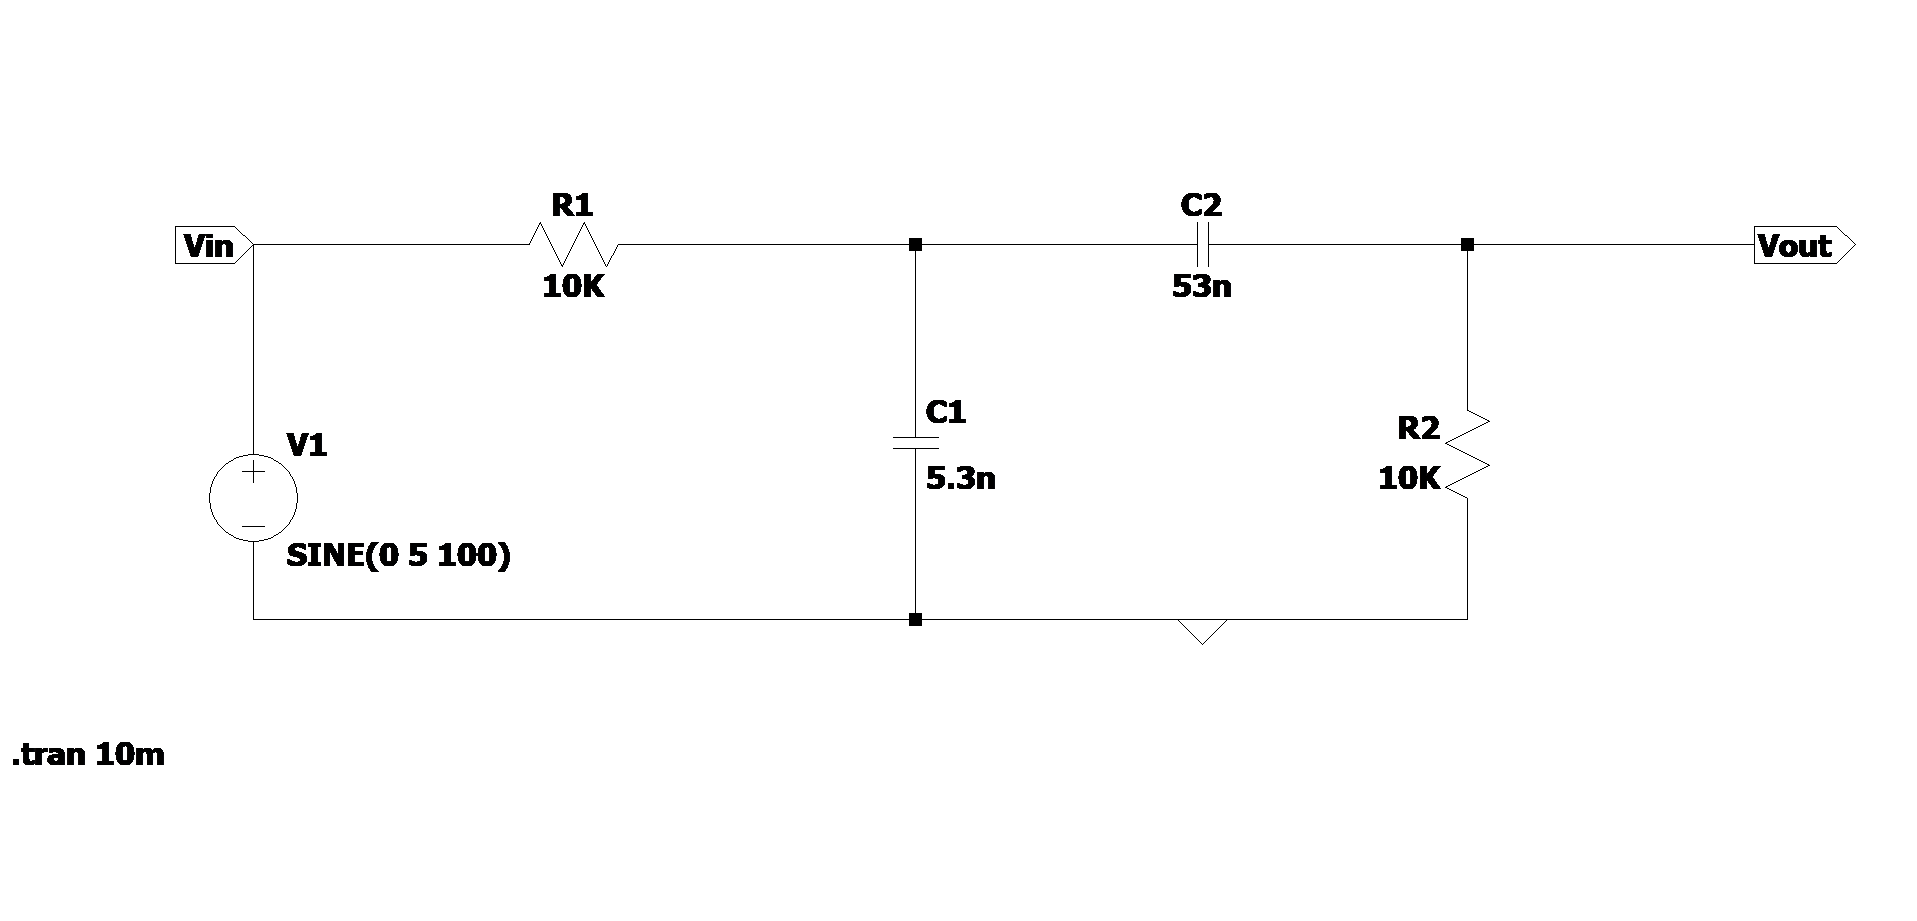
\includegraphics[width=0.85\textwidth]{lab06-part1.png}
    \caption{Passive bandpass filter: low-pass stage cascaded directly into the high-pass stage.}
\end{figure}

\begin{lstlisting}[style=netlist, caption={LTSpice netlist: passive cascade}]
* /Users/abdonmorales/Library/CloudStorage/OneDrive-TheUniversityofTexasatAustin/Summer 2026/ECE 402/Lab Notes/Lab 06/lab06-part1.asc
* Generated by LTspice 26.0.2 for MacOS.
V1 Vin 0 SINE(0 5 100)
R1 N001 Vin 10K
R2 0 Vout 10K
C1 N001 0 5.3n
C2 Vout N001 53n
.tran 10m
.backanno
.end
\end{lstlisting}

\begin{figure}[H]
    \centering
    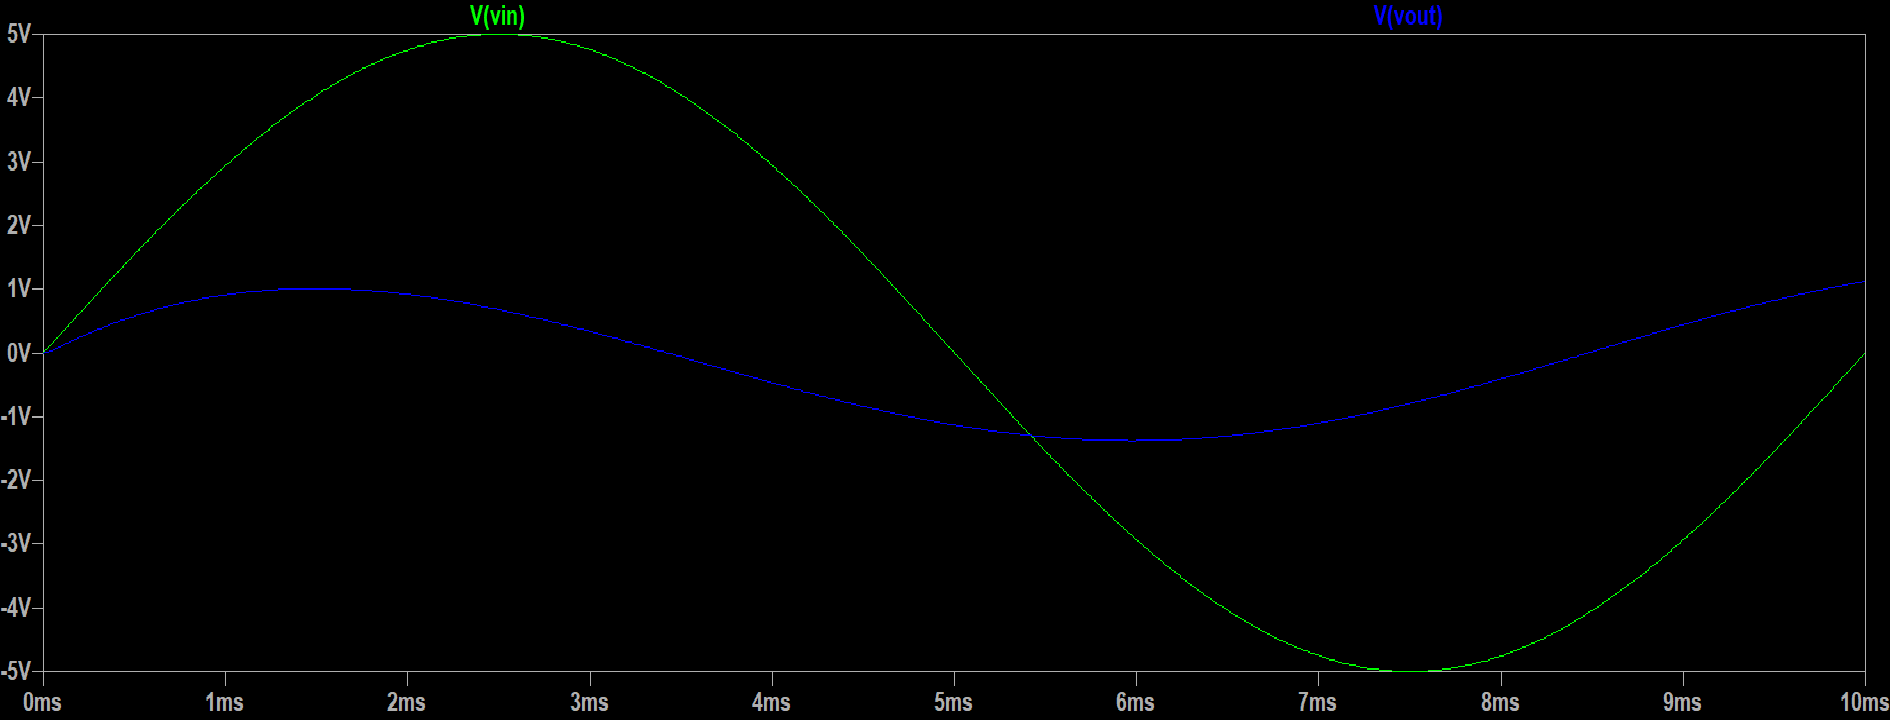
\includegraphics[width=0.95\textwidth]{lab06-part1-waveform.png}
    \caption{Input signal (green) and high-pass output (blue) for the passive cascade.}
\end{figure}

\subsection*{Isolated (op-amp buffered) bandpass filter}

\begin{figure}[H]
    \centering
    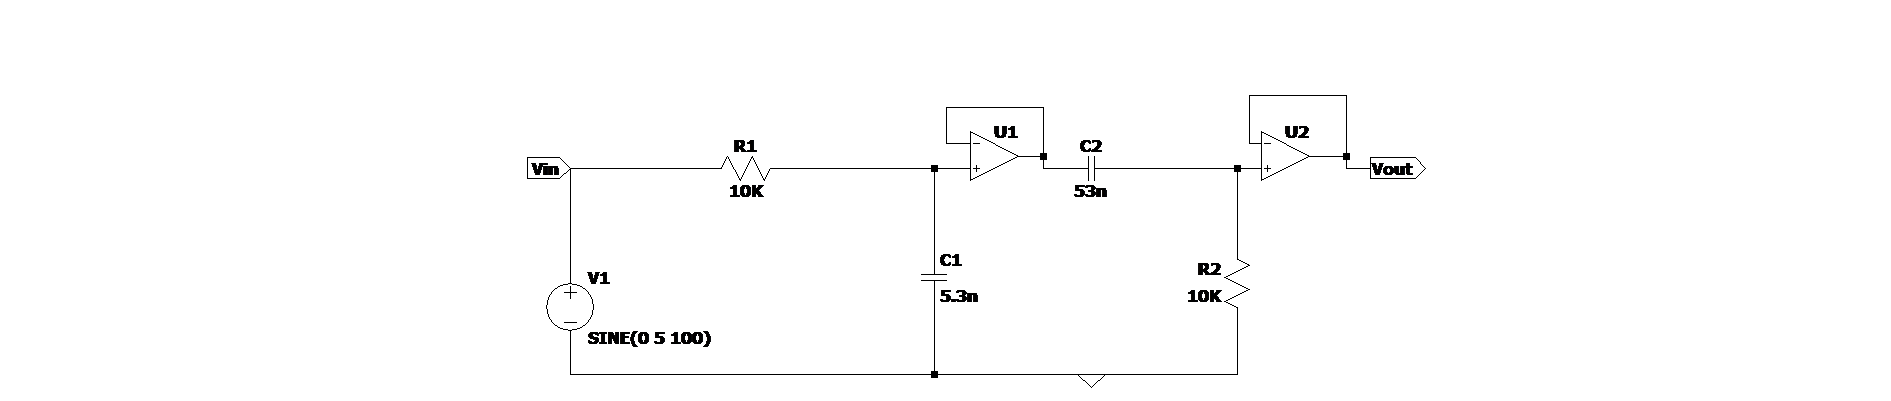
\includegraphics[width=0.95\textwidth]{lab06-part2.png}
    \caption{Buffered bandpass filter: unity-gain op-amps isolate the two stages.}
\end{figure}

\begin{lstlisting}[style=netlist, caption={LTSpice netlist: op-amp buffered version}]
* /Users/abdonmorales/Library/CloudStorage/OneDrive-TheUniversityofTexasatAustin/Summer 2026/ECE 402/Lab Notes/Lab 06/lab06-part2.asc
* Generated by LTspice 26.0.2 for MacOS.
V1 Vin 0 SINE(0 5 100)
R1 N002 Vin 10K
R2 0 N003 10K
C1 N002 0 5.3n
C2 N003 N001 53n
U1 N001 N002 N001 opamp Aol=100K GBW=10Meg
U2 Vout N003 Vout opamp Aol=100K GBW=10Meg
.tran 10m
.inc opamp.sub
.backanno
.end
\end{lstlisting}

\begin{figure}[H]
    \centering
    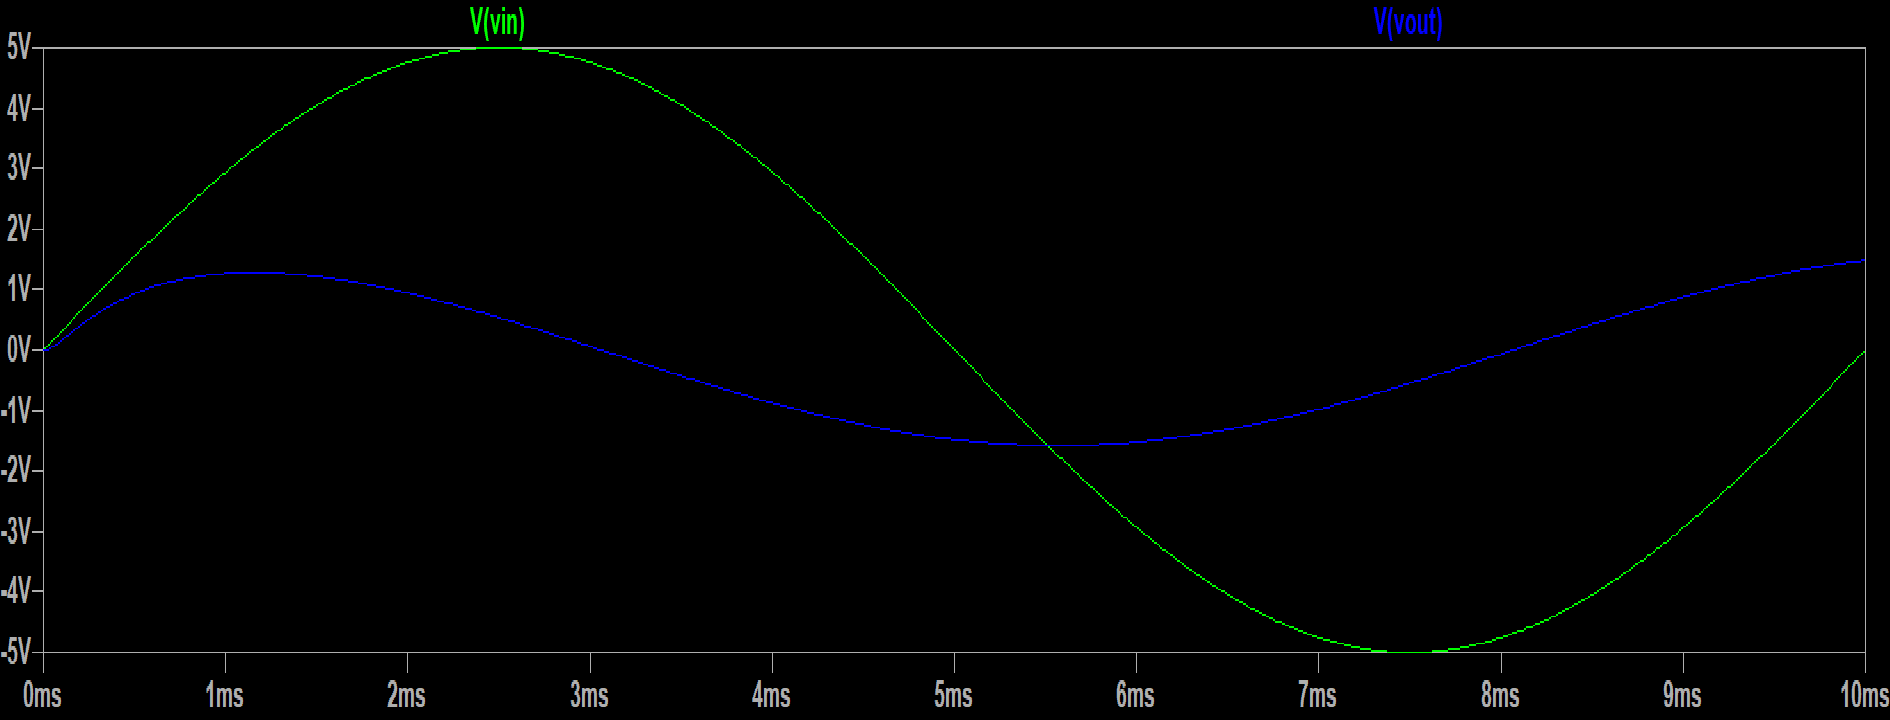
\includegraphics[width=0.95\textwidth]{lab06-part2-waveform.png}
    \caption{Input signal (green) and output (blue) for the buffered version.}
\end{figure}

The peak output from each run is tabulated next to the measured bench data in the
Measurements section for direct comparison. These simulations use the calculated caps
(\SI{5.3}{\nano\farad} and \SI{53}{\nano\farad}) shown in the netlists above, while the
bench used the stock \SI{4.7}{\nano\farad} and \SI{47}{\nano\farad} parts.

%------------------------------------------------------------------------------
\section*{Measurements}

The peak output voltage at each test frequency is below for both builds, with the
LTSpice value and the bench value side by side. The simulation used the calculated
caps (\SI{5.3}{\nano\farad} and \SI{53}{\nano\farad}); the bench build used the
stock parts (\SI{4.7}{\nano\farad} and \SI{47}{\nano\farad}). The last column is the
percent difference of the measured value relative to the simulation.

\begin{table}[H]
    \centering
    \caption{Circuit 1: passive cascade (no op-amps), \(V_{in} = \SI{5}{\volt}\)}
    \begin{tabular}{lccc}
        \toprule
        Frequency & \(V_{out}\) simulated (V) & \(V_{out}\) measured (V) & Diff.\ (\%) \\
        \midrule
        \SI{100}{\hertz}   & 1.101 & 1.24 & $+12.6$ \\
        \SI{300}{\hertz}   & 2.164 & 2.08 & $-3.9$ \\
        \SI{500}{\hertz}   & 2.305 & 2.26 & $-2.0$ \\
        \SI{1}{\kilo\hertz}   & 2.340 & 2.32 & $-0.9$ \\
        \SI{3}{\kilo\hertz}   & 2.153 & 2.16 & $+0.3$ \\
        \SI{5}{\kilo\hertz}   & 1.820 & 1.90 & $+4.4$ \\
        \SI{10}{\kilo\hertz}  & 1.209 & 1.40 & $+15.8$ \\
        \SI{100}{\kilo\hertz} & 0.136 & 0.32 & $+135.6$ \\
        \bottomrule
    \end{tabular}
\end{table}

\begin{table}[H]
    \centering
    \caption{Circuit 2: buffered version (unity-gain op-amps), \(V_{in} = \SI{5}{\volt}\)}
    \begin{tabular}{lccc}
        \toprule
        Frequency & \(V_{out}\) simulated (V) & \(V_{out}\) measured (V) & Diff.\ (\%) \\
        \midrule
        \SI{100}{\hertz}   & 1.452 & 1.34 & $-7.7$ \\
        \SI{300}{\hertz}   & 3.500 & 3.14 & $-10.3$ \\
        \SI{500}{\hertz}   & 4.184 & 3.54 & $-15.4$ \\
        \SI{1}{\kilo\hertz}   & 4.447 & 3.76 & $-15.4$ \\
        \SI{3}{\kilo\hertz}   & 3.500 & 3.30 & $-5.7$ \\
        \SI{5}{\kilo\hertz}   & 2.446 & 2.54 & $+3.8$ \\
        \SI{10}{\kilo\hertz}  & 1.333 & 1.44 & $+8.0$ \\
        \SI{100}{\kilo\hertz} & 0.135 & 0.24 & $+77.8$ \\
        \bottomrule
    \end{tabular}
\end{table}

Both circuits peak at \SI{1}{\kilo\hertz}, near the geometric center of the band, which
is what a bandpass response should do. The passive cascade peaks at about
\SI{2.3}{\volt} while the buffered version reaches about \SI{3.8}{\volt} on the bench
(\SI{4.4}{\volt} in simulation), so adding the op-amps roughly doubles the passband
output.

%------------------------------------------------------------------------------
\section*{Observations \& Discussion}

There was a clear difference between the two circuits, and the cause is loading.
In the passive cascade the high-pass stage draws current directly from the low-pass
output, so the first stage is loaded down and the passband peaks at only about
\SI{2.3}{\volt}. Adding the unity-gain op-amps isolates the stages and approximately
doubles this output, reaching about \SI{3.8}{\volt} on the bench and \SI{4.4}{\volt}
in simulation, because each buffer presents a high input impedance to the preceding
stage and a low output impedance to the following one. Both versions peak at
\SI{1}{\kilo\hertz}, the center of the band, which is the expected behavior for a
bandpass response. Which circuit matched expectation depends on the reference used:
the passive build agreed closely with its own simulation, within about five percent
from \SI{300}{\hertz} to \SI{5}{\kilo\hertz}, while the buffered build reproduced the
ideal textbook bandpass shape more faithfully (a taller, cleaner peak) but fell about
ten to fifteen percent below the ideal simulation across the passband. This shortfall
represents the primary cost of the op-amps and is attributable to the real 741
limitations (finite gain-bandwidth, input bias, and offset) that the LTSpice model
does not capture, in addition to the two extra components and the
\(\pm\SI{12}{\volt}\) rails they require. For a voice-band filter the tradeoff is
justified, since the passive version discards a substantial portion of the in-band
signal.

The main concern appeared at \SI{100}{\kilo\hertz}, where both bench readings
(\SI{0.32}{\volt} passive and \SI{0.24}{\volt} buffered) remained well above the
simulated floor of about \SI{0.14}{\volt}. The physical breadboard does not attenuate
out-of-band signals as effectively as the ideal model, which we attribute to
high-frequency feedthrough through parasitic capacitance in the board and probes. The
buffered measurements also fell uniformly below simulation across the passband,
whereas the passive measurements straddled it. This offset reflects error introduced
by the op-amps, which the purely passive circuit does not have. The capacitor
substitution shifted the band as well. The design called for \SI{5.31}{\nano\farad}
and \SI{53.05}{\nano\farad}, which is what we simulated, but these are not standard
values, so the bench build used \SI{4.7}{\nano\farad} and \SI{47}{\nano\farad}.
Smaller capacitance raises the cutoff frequency, so both edges moved up: the low-pass
corner went from \SI{3}{\kilo\hertz} to about \SI{3.39}{\kilo\hertz} and the high-pass
corner from \SI{300}{\hertz} to about \SI{339}{\hertz}, which widened the passband
slightly and shifted it up by approximately thirteen percent on each edge. This
component-value difference, together with resistor and capacitor tolerances, partly
explains the gap between the measured and simulated values, though for voice filtering
the shift is negligible.

%==============================================================================
\end{document}